
%%--------------------------------------------------
%% Serway: Physics for Scientists and Engineers
%%--------------------------------------------------


%% Chapter 08: Potential Energy
%%--------------------------------------------------


%% Table of Contents
%%--------------------------------------------------

%% 8.1 The Nonisolated System: Conservation of Energy
%% 8.2 The Isolated System
%% 8.3 Situations Involving Kinetic Friction
%% 8.4 Changes in Mechanical Energy for Nonconservative Forces
%% 8.5 Power


%% Serway Multiple Choice Questions
%%--------------------------------------------------
\element{serway-mc}{
\begin{question}{serway-ch08-q01}
    A single conservative force $F_x=(6.0x - 12)\,\si{\newton}$
        ($x$ is in meters) acts on a particle moving along the $x$ axis. 
    The potential energy associated with this force is assigned a value of \SI{+20}{\joule} at $x=0$.
    What is the potential energy at $x=\SI{3.0}{\meter}$?
    \begin{multicols}{3}
    \begin{choices}
        \wrongchoice{\SI{+11}{\joule}}
      \correctchoice{\SI{+29}{\joule}}
        \wrongchoice{\SI{+9.0}{\joule}}
        \wrongchoice{\SI{-9.0}{\joule}}
        \wrongchoice{\SI{+20}{\joule}}
    \end{choices}
    \end{multicols}
\end{question}
}

\element{serway-mc}{
\begin{question}{serway-ch08-q02}
    As a particle moves along the $x$ axis it is acted upon by a single conservative force given by $F_x=(20-4.0x)\,\si{\newton}$ where $x$ is in meters.
    The potential energy associated with this force has the value \SI{+30}{\joule} at the origin ($x=0$). 
    What is the value of the potential energy at $x=\SI{4.0}{\meter}$?
    \begin{multicols}{3}
    \begin{choices}
        \wrongchoice{\SI{-48}{\joule}}
        \wrongchoice{\SI{+78}{\joule}}
      \correctchoice{\SI{-18}{\joule}}
        \wrongchoice{\SI{+48}{\joule}}
        \wrongchoice{\SI{+80}{\joule}}
    \end{choices}
    \end{multicols}
\end{question}
}

\element{serway-mc}{
\begin{question}{serway-ch08-q03}
    A \SI{0.40}{\kilo\gram} particle moves under the influence of a single conservative force.
    At point $A$ where the particle has a speed of \SI{10}{\meter\per\second},
        the potential energy associated with the conservative force is \SI{+40}{\joule}. 
    As the particle moves from $A$ to $B$,
        the force does \SI{+25}{\joule} of work on the particle. 
    What is the value of the potential energy at point B?
    \begin{multicols}{3}
    \begin{choices}
        \wrongchoice{\SI{+65}{\joule}}
      \correctchoice{\SI{+15}{\joule}}
        \wrongchoice{\SI{+35}{\joule}}
        \wrongchoice{\SI{+45}{\joule}}
        \wrongchoice{\SI{-40}{\joule}}
    \end{choices}
    \end{multicols}
\end{question}
}

\element{serway-mc}{
\begin{question}{serway-ch08-q04}
    As a \SI{1.0}{\kilo\gram} object moves from point $A$ to point $B$,
        it is acted upon by a single conservative force which does \SI{-40}{\joule} of work during this motion. 
    At point $A$ the speed of the particle is \SI{6.0}{\meter\per\second} and the potential energy associated with the force is \SI{+50}{\joule}. 
    What is the potential energy at point $B$?
    \begin{multicols}{3}
    \begin{choices}
        \wrongchoice{\SI{+72}{\joule}}
        \wrongchoice{\SI{+10}{\joule}}
      \correctchoice{\SI{+90}{\joule}}
        \wrongchoice{\SI{+28}{\joule}}
        \wrongchoice{\SI{+68}{\joule}}
    \end{choices}
    \end{multicols}
\end{question}
}

\element{serway-mc}{
\begin{question}{serway-ch08-q05}
    A \SI{12}{\kilo\gram} block on a horizontal frictionless surface is attached to a light spring (force constant = \SI{0.80}{\kilo\newton\per\meter}). 
    The block is initially at rest at its equilibrium position when a force (magnitude $P=\SI{80}{\newton}$) acting parallel to the surface is applied to the block,
        as shown. 
    \begin{center}
    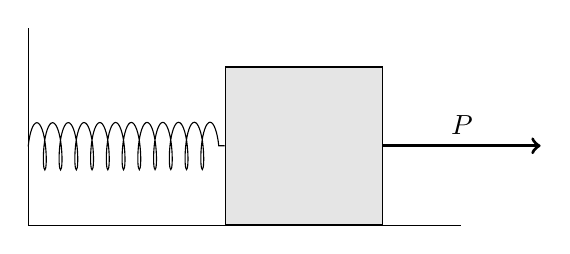
\begin{tikzpicture}
        \draw (0,2.5) -- (0,0) -- (5.5,0);
        \node[fill=white!90!black,draw,rectangle,minimum size=2cm,anchor=south] (M) at (3.5,0) {};
        \draw[decoration={aspect=0.2,segment length=2.0mm,amplitude=3mm,coil},decorate] (0,1) -- (M.west);
        \draw[very thick,->] (M.east) -- +(0:2) node[pos=0.5,anchor=south] {$P$};
    \end{tikzpicture}
    \end{center}
    What is the speed of the block when it is \SI{13}{\centi\meter} from its equilibrium position?
    \begin{multicols}{3}
    \begin{choices}
      \correctchoice{\SI{0.78}{\meter\per\second}}
        \wrongchoice{\SI{0.81}{\meter\per\second}}
        \wrongchoice{\SI{0.71}{\meter\per\second}}
        \wrongchoice{\SI{0.58}{\meter\per\second}}
        \wrongchoice{\SI{0.64}{\meter\per\second}}
    \end{choices}
    \end{multicols}
\end{question}
}

\element{serway-mc}{
\begin{question}{serway-ch08-q06}
    A \SI{7.0}{\kilo\gram} block on a horizontal frictionless surface is attached to a light spring (force constant = \SI{1.2}{\kilo\newton\per\meter}). 
    The block is initially at rest at its equilibrium position when a force of magnitude P acting parallel to the surface is applied to the block, as shown. 
    \begin{center}
    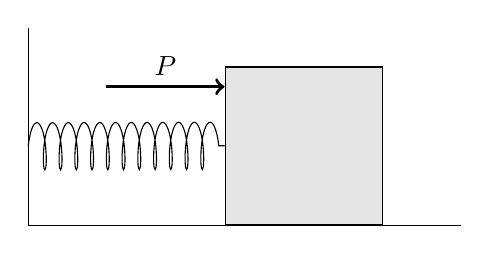
\begin{tikzpicture}
        \draw (0,2.5) -- (0,0) -- (5.5,0);
        \node[fill=white!90!black,draw,rectangle,minimum size=2cm,anchor=south] (M) at (3.5,0) {};
        \draw[decoration={aspect=0.2,segment length=2.0mm,amplitude=3mm,coil},decorate] (0,1) -- (M.west);
        \draw[very thick,<-] (M.west) ++ (90:0.75) -- ++(180:1.5) node[anchor=south,pos=0.5] {$P$};
    \end{tikzpicture}
    \end{center}
    When the block is \SI{8.0}{\centi\meter} from the equilibrium position,
        it has a speed of \SI{0.80}{\meter\per\second}. 
    How much work is done on the block by the force $P$ as the block moves the \SI{8.0}{\centi\meter}?
    \begin{multicols}{3}
    \begin{choices}
        \wrongchoice{\SI{7.4}{\joule}}
        \wrongchoice{\SI{5.4}{\joule}}
      \correctchoice{\SI{6.1}{\joule}}
        \wrongchoice{\SI{6.7}{\joule}}
        \wrongchoice{\SI{4.9}{\joule}}
    \end{choices}
    \end{multicols}
\end{question}
}

\element{serway-mc}{
\begin{question}{serway-ch08-q07}
    A \SI{0.60}{\kilo\gram} object is suspended from the ceiling at the end of a \SI{2.0}{\meter} string. 
    When pulled to the side and released,
        it has a speed of \SI{4.0}{\meter\per\second} at the lowest point of its path. 
    What maximum angle does the string make with the vertical as the object swings up?
    \begin{multicols}{3}
    \begin{choices}
        \wrongchoice{\ang{61}}
      \correctchoice{\ang{54}}
        \wrongchoice{\ang{69}}
        \wrongchoice{\ang{77}}
        \wrongchoice{\ang{47}}
    \end{choices}
    \end{multicols}
\end{question}
}

\element{serway-mc}{
\begin{question}{serway-ch08-q08}
    A pendulum is made by letting a \SI{2.0}{\kilo\gram} object swing at the end of a string that has a length of \SI{1.5}{\meter}. 
    The maximum angle the string makes with the vertical as the pendulum swings is \ang{30}. 
    What is the speed of the object at the lowest point in its trajectory?
    \begin{multicols}{3}
    \begin{choices}
      \correctchoice{\SI{2.0}{\meter\per\second}}
        \wrongchoice{\SI{2.2}{\meter\per\second}}
        \wrongchoice{\SI{2.5}{\meter\per\second}}
        \wrongchoice{\SI{2.7}{\meter\per\second}}
        \wrongchoice{\SI{3.1}{\meter\per\second}}
    \end{choices}
    \end{multicols}
\end{question}
}

\element{serway-mc}{
\begin{question}{serway-ch08-q09}
    A \SI{2.0}{\kilo\gram} mass swings at the end of a light string (length = \SI{3.0}{\meter}).
    Its speed at the lowest point on its circular path is \SI{6.0}{\meter\per\second}. 
    What is its kinetic energy at an instant when the string makes an angle of \ang{50} with the vertical?
    \begin{multicols}{3}
    \begin{choices}
        \wrongchoice{\SI{21}{\joule}}
      \correctchoice{\SI{15}{\joule}}
        \wrongchoice{\SI{28}{\joule}}
        \wrongchoice{\SI{36}{\joule}}
        \wrongchoice{\SI{23}{\joule}}
    \end{choices}
    \end{multicols}
\end{question}
}

\element{serway-mc}{
\begin{question}{serway-ch08-q10}
    A \SI{2.5}{\kilo\gram} object suspended from the ceiling by a string that has a length of \SI{2.5}{\meter} is released from rest with the string \ang{40} below the horizontal position. 
    What is the tension in the string at the instant when the object passes through its lowest position?
    \begin{multicols}{3}
    \begin{choices}
        \wrongchoice{\SI{11}{\newton}}
        \wrongchoice{\SI{25}{\newton}}
      \correctchoice{\SI{42}{\newton}}
        \wrongchoice{\SI{18}{\newton}}
        \wrongchoice{\SI{32}{\newton}}
    \end{choices}
    \end{multicols}
\end{question}
}

\element{serway-mc}{
\begin{question}{serway-ch08-q11}
    A certain pendulum consists of a \SI{1.5}{\kilo\gram} mass swinging at the end of a string (length = \SI{2.0}{\meter}). 
    At the lowest point in the swing the tension in the string is equal to \SI{20}{\newton}. 
    To what maximum height above this lowest point will the mass rise during its oscillation?
    \begin{multicols}{3}
    \begin{choices}
        \wrongchoice{\SI{77}{\centi\meter}}
        \wrongchoice{\SI{50}{\centi\meter}}
        \wrongchoice{\SI{63}{\centi\meter}}
      \correctchoice{\SI{36}{\centi\meter}}
        \wrongchoice{\SI{95}{\centi\meter}}
    \end{choices}
    \end{multicols}
\end{question}
}

\element{serway-mc}{
\begin{question}{serway-ch08-q12}
    A \SI{0.80}{\kilo\gram} object tied to the end of a \SI{2.0}{\meter} string swings as a pendulum. 
    At the lowest point of its swing,
        the object has a kinetic energy of \SI{10}{\joule}. 
    Determine the speed of the object at the instant when the string makes an angle of \ang{50} with the vertical.
    \begin{multicols}{3}
    \begin{choices}
        \wrongchoice{\SI{5.6}{\meter\per\second}}
        \wrongchoice{\SI{4.4}{\meter\per\second}}
      \correctchoice{\SI{3.3}{\meter\per\second}}
        \wrongchoice{\SI{5.0}{\meter\per\second}}
        \wrongchoice{\SI{6.1}{\meter\per\second}}
    \end{choices}
    \end{multicols}
\end{question}
}

\element{serway-mc}{
\begin{question}{serway-ch08-q13}
    A \SI{0.04}{\kilo\gram} ball is thrown from the top of a \SI{30}{\meter} tall building (point $A$) at an unknown angle above the horizontal.
    As shown in the figure,
        the ball attains a maximum height of \SI{10}{\meter} above the top of the building before striking the ground at point $B$.
    \begin{center}
    \begin{tikzpicture}
        %% Surface
        \draw (-1,0) -- (0,0) -- (0,-3) -- (5,-3);
        \draw[dashed] (0,0) -- (3,0);
        %% Labels
        \draw[<->] (2,0) -- (2,1) node[pos=0.5,anchor=center,fill=white] {\SI{10}{\meter}};
        \draw[<->] (2,0) -- (2,-3) node[pos=0.5,anchor=center,fill=white] {\SI{30}{\meter}};
        %% Trajectory
        \draw[dashed] (0,0) parabola bend (2,1) (4,-3);
        \draw[fill] (0,0) circle (1.5pt) node[anchor=south east] {$A$};
        %% Vectors
        \draw[very thick,->] (0,0) -- ++(40:0.5);
        \draw[fill] (4,-3) circle (1.5pt) node[anchor=south west] {$B$};
        \draw[very thick,<-] (4,-3) -- ++(102:0.5);
    \end{tikzpicture}
    \end{center}
    If air resistance is negligible,
        what is the value of the kinetic energy of the ball at $B$ minus the kinetic energy of the ball at $A(K_B-K_A)$?
    \begin{multicols}{3}
    \begin{choices}
      \correctchoice{\SI{12}{\joule}}
        \wrongchoice{\SI{-12}{\joule}}
        \wrongchoice{\SI{20}{\joule}}
        \wrongchoice{\SI{-20}{\joule}}
        \wrongchoice{\SI{32}{\joule}}
    \end{choices}
    \end{multicols}
\end{question}
}

\element{serway-mc}{
\begin{question}{serway-ch08-q14}
    A \SI{1.2}{\kilo\gram} mass is projected from ground level with a velocity of \SI{30}{\meter\per\second} at some unknown angle above the horizontal.
    A short time after being projected,
        the mass barely clears a \SI{16}{\meter} tall fence. 
    Disregard air resistance and assume the ground is level. 
    What is the kinetic energy of the mass as it clears the fence?
    \begin{multicols}{3}
    \begin{choices}
      \correctchoice{\SI{0.35}{\kilo\joule}}
        \wrongchoice{\SI{0.73}{\kilo\joule}}
        \wrongchoice{\SI{0.40}{\kilo\joule}}
        \wrongchoice{\SI{0.68}{\kilo\joule}}
        \wrongchoice{\SI{0.19}{\kilo\joule}}
    \end{choices}
    \end{multicols}
\end{question}
}

\element{serway-mc}{
\begin{question}{serway-ch08-q15}
    A \SI{2.0}{\kilo\gram} mass is projected from the edge of the top of a \SI{20}{\meter} tall building with a velocity of \SI{24}{\meter\per\second} at some unknown angle above the horizontal. 
    Disregard air resistance and assume the ground is level. 
    What is the kinetic energy of the mass just before it strikes the ground?
    \begin{multicols}{3}
    \begin{choices}
        \wrongchoice{\SI{0.18}{\kilo\joule}}
      \correctchoice{\SI{0.97}{\kilo\joule}}
        \wrongchoice{\SI{0.89}{\kilo\joule}}
        \wrongchoice{\SI{0.26}{\kilo\joule}}
        \wrongchoice{\SI{0.40}{\kilo\joule}}
    \end{choices}
    \end{multicols}
\end{question}
}

\element{serway-mc}{
\begin{question}{serway-ch08-q16}
    A skier weighing \SI{0.70}{\kilo\newton} goes over a frictionless circular hill as shown.
    \begin{center}
    \begin{tikzpicture}
        %% Surface
        \draw (135:3) arc(135:45:3);
        \draw (135:3) -- ++(225:2);
        \draw (45:3) -- ++(315:2);
        %% Vectors
        \draw[dashed] (0,0)  -- (135:3);
        \draw[<->] (135:2) arc (135:90:2) node[fill=white,anchor=center,pos=0.5] {\ang{45}}; 
        \draw[thick,->] (0,0) -- ++(90:3) node[pos=0.3,anchor=center,fill=white] {\SI{10}{\meter}};
        %% Labels
        \draw[fill] (135:3) circle (1.5pt) node[anchor=south east] {$A$};
        \draw[fill] (90:3) circle (1.5pt) node[anchor=south east] {$B$};
    \end{tikzpicture}
    \end{center}
    If the skier's speed at point $A$ is \SI{9.2}{\meter\per\second},
        what is his speed at the top of the hill (point $B$)?
    \begin{multicols}{3}
    \begin{choices}
        \wrongchoice{\SI{3.1}{\meter\per\second}}
        \wrongchoice{\SI{6.2}{\meter\per\second}}
      \correctchoice{\SI{5.2}{\meter\per\second}}
        \wrongchoice{\SI{4.1}{\meter\per\second}}
        \wrongchoice{\SI{6.5}{\meter\per\second}}
    \end{choices}
    \end{multicols}
\end{question}
}

\element{serway-mc}{
\begin{question}{serway-ch08-q17}
    A skier weighing \SI{0.80}{\kilo\newton} comes down a frictionless ski run that is circular ($R=\SI{30}{\meter}$) at the bottom, as shown.
    \begin{center}
    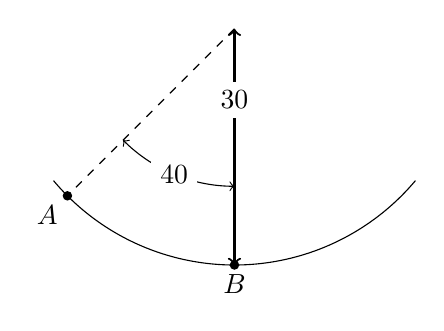
\begin{tikzpicture}
        %% Surface
        \draw (220:3) arc(220:320:3);
        %% Vectors
        \draw[dashed] (0,0)  -- (225:3);
        \draw[<->] (225:2) arc (225:270:2) node[fill=white,anchor=center,pos=0.5] {\ang{40}}; 
        \draw[thick,<->] (0,0) -- ++(270:3) node[pos=0.3,anchor=center,fill=white] {\SI{30}{\meter}};
        %% Labels
        \draw[fill] (225:3) circle (1.5pt) node[anchor=north east] {$A$};
        \draw[fill] (270:3) circle (1.5pt) node[anchor=north] {$B$};
    \end{tikzpicture}
    \end{center}
    If her speed is \SI{12}{\meter\per\second} at point $A$,
        what is her speed at the bottom of the hill (point $B$)?
    \begin{multicols}{3}
    \begin{choices}
      \correctchoice{\SI{17}{\meter\per\second}}
        \wrongchoice{\SI{19}{\meter\per\second}}
        \wrongchoice{\SI{18}{\meter\per\second}}
        \wrongchoice{\SI{20}{\meter\per\second}}
        \wrongchoice{\SI{12}{\meter\per\second}}
    \end{choices}
    \end{multicols}
\end{question}
}

\element{serway-mc}{
\begin{question}{serway-ch08-q18}
    A spring ($k=\SI{600}{\newton\per\meter}$) is placed in a vertical position with its lower end supported by a horizontal surface. 
    The upper end is depressed \SI{20}{\centi\meter},
        and a \SI{4.0}{\kilo\gram} block is placed on the depressed spring. 
    The system is then released from rest. 
    How far above the point of release will the block rise?
    \begin{multicols}{3}
    \begin{choices}
        \wrongchoice{\SI{46}{\centi\meter}}
        \wrongchoice{\SI{36}{\centi\meter}}
        \wrongchoice{\SI{41}{\centi\meter}}
      \correctchoice{\SI{31}{\centi\meter}}
        \wrongchoice{\SI{20}{\centi\meter}}
    \end{choices}
    \end{multicols}
\end{question}
}

\element{serway-mc}{
\begin{question}{serway-ch08-q19}
    A spring ($k=\SI{200}{\newton\per\meter}$) is suspended with its upper end supported from a ceiling. 
    With the spring hanging in its equilibrium configuration,
        an object (mass = \SI{2.0}{\kilo\gram}) is attached to the lower end and released from rest. 
    What is the speed of the object after it has fallen \SI{4.0}{\centi\meter}?
    \begin{multicols}{3}
    \begin{choices}
        \wrongchoice{\SI{90}{\centi\meter\per\second}}
      \correctchoice{\SI{79}{\centi\meter\per\second}}
        \wrongchoice{\SI{96}{\centi\meter\per\second}}
        \wrongchoice{\SI{83}{\centi\meter\per\second}}
        \wrongchoice{\SI{57}{\centi\meter\per\second}}
    \end{choices}
    \end{multicols}
\end{question}
}

\element{serway-mc}{
\begin{question}{serway-ch08-q20}
    A \SI{2.0}{\kilo\gram} block sliding on a horizontal frictionless surface is attached to one end of a horizontal spring ($k=\SI{200}{\newton\per\meter}$) which has its other end fixed. 
    If the block has a speed of \SI{4.0}{\meter\per\second} as it passes through the equilibrium position,
        what is its speed when it is \SI{20}{\centi\meter} from the equilibrium position?
    \begin{multicols}{3}
    \begin{choices}
        \wrongchoice{\SI{2.6}{\meter\per\second}}
        \wrongchoice{\SI{3.1}{\meter\per\second}}
      \correctchoice{\SI{3.5}{\meter\per\second}}
        \wrongchoice{\SI{1.9}{\meter\per\second}}
        \wrongchoice{\SI{2.3}{\meter\per\second}}
    \end{choices}
    \end{multicols}
\end{question}
}

\element{serway-mc}{
\begin{question}{serway-ch08-q21}
    A block (mass = \SI{4.0}{\kilo\gram}) sliding on a horizontal frictionless surface is attached to one end of a horizontal spring ($k=\SI{100}{\newton\per\meter}$) which has its other end fixed.
    If the maximum distance the block slides from the equilibrium position is equal to \SI{20}{\centi\meter},
        what is the speed of the block at an instant when it is a distance of \SI{16}{\centi\meter} from the equilibrium position?
    \begin{multicols}{3}
    \begin{choices}
        \wrongchoice{\SI{71}{\centi\meter\per\second}}
      \correctchoice{\SI{60}{\centi\meter\per\second}}
        \wrongchoice{\SI{80}{\centi\meter\per\second}}
        \wrongchoice{\SI{87}{\centi\meter\per\second}}
        \wrongchoice{\SI{57}{\centi\meter\per\second}}
    \end{choices}
    \end{multicols}
\end{question}
}

\element{serway-mc}{
\begin{question}{serway-ch08-q22}
    A \SI{1.0}{\kilo\gram} block is released from rest at the top of a frictionless incline that makes an angle of \ang{37} with the horizontal. 
    An unknown distance down the incline from the point of release, there is a spring with $k=\SI{200}{\newton\per\meter}$.
    It is observed that the mass is brought momentarily to rest after compressing the spring \SI{0.20}{\meter}. 
    How far does the mass slide from the point of release until it is brought momentarily to rest?
    \begin{multicols}{3}
    \begin{choices}
        \wrongchoice{\SI{0.98}{\meter}}
      \correctchoice{\SI{0.68}{\meter}}
        \wrongchoice{\SI{0.82}{\meter}}
        \wrongchoice{\SI{0.55}{\meter}}
        \wrongchoice{\SI{0.20}{\meter}}
    \end{choices}
    \end{multicols}
\end{question}
}

\element{serway-mc}{
\begin{question}{serway-ch08-q23}
    A \SI{20}{\kilo\gram} mass is fastened to a light spring ($k=\SI{380}{\newton\per\meter}$) that passes over a pulley as shown. 
    \begin{center}
    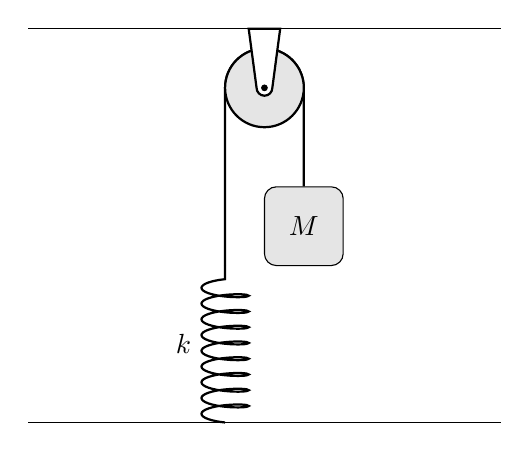
\begin{tikzpicture}
        %% Top and Bottom
        \draw (-3,0) -- (3,0);
        \draw (-3,-5) -- (3,-5);
        %% Mass
        \node[draw,fill=white!90!black,rectangle,rounded corners=1ex,minimum size=1cm,anchor=north] (M) at (0.5,-2) {$M$};
        %% Spring and Rope
        \draw[thick,decoration={aspect=0.2,segment length=2.0mm,amplitude=3mm,coil},decorate] (-0.5,-5) -- (-0.5,-3) node[pos=0.5,xshift=-3mm,anchor=east] {$k$};
        \draw[thick] (-0.5,-3) -- (-0.5,-0.75) arc(180:0:0.5) -- (0.5,-2);
        %% Pulley
        %\draw[thick] (A.south east) ++(90:0.5) -- (0.75,0.5) arc(90:0:0.25) -- (B.north);
        \draw[thick,fill=white!90!black] (0,-0.75) circle (0.50);
        \draw[thick,fill=white] (-0.2,0) -- (-0.1,-0.75) arc(180:360:0.1) -- (0.2,0) -- cycle;
        \draw[fill] (0,-0.75) circle (1pt);
    \end{tikzpicture}
    \end{center}
    The pulley is frictionless,
        and the mass is released from rest when the spring is unstretched. 
    After the mass has dropped \SI{0.40}{\meter}, what is its speed?
    \begin{multicols}{3}
    \begin{choices}
      \correctchoice{\SI{2.2}{\meter\per\second}}
        \wrongchoice{\SI{2.5}{\meter\per\second}}
        \wrongchoice{\SI{1.9}{\meter\per\second}}
        \wrongchoice{\SI{1.5}{\meter\per\second}}
        \wrongchoice{\SI{3.6}{\meter\per\second}}
    \end{choices}
    \end{multicols}
\end{question}
}

\element{serway-mc}{
\begin{question}{serway-ch08-q24}
    A spring ($k=\SI{600}{\newton\per\meter}$) is at the bottom of a frictionless plane that makes an angle of \ang{30} with the horizontal. 
    The upper end of the spring is depressed \SI{0.10}{\meter},
        and a \SI{2.0}{\kilo\gram} block is placed against the depressed spring. 
    The system is then released from rest. 
    What is the kinetic energy of the block at the instant it has traveled \SI{0.10}{\meter} and the spring has returned to its uncompressed length?
    \begin{multicols}{3}
    \begin{choices}
      \correctchoice{\SI{2.0}{\joule}}
        \wrongchoice{\SI{1.8}{\joule}}
        \wrongchoice{\SI{2.2}{\joule}}
        \wrongchoice{\SI{1.6}{\joule}}
        \wrongchoice{\SI{1.0}{\joule}}
    \end{choices}
    \end{multicols}
\end{question}
}

\element{serway-mc}{
\begin{question}{serway-ch08-q25}
    A spring ($k=\SI{600}{\newton\per\meter}$) is placed in a vertical position with its lower end supported by a horizontal surface. 
    A \SI{2.0}{\kilo\gram} block that is initially \SI{0.40}{\meter} above the upper end of the spring is dropped from rest onto the spring. 
    What is the kinetic energy of the block at the instant it has fallen \SI{0.50}{\meter}
        (compressing the spring \SI{0.10}{\meter})?
    \begin{multicols}{3}
    \begin{choices}
        \wrongchoice{\SI{5.3}{\joule}}
      \correctchoice{\SI{6.8}{\joule}}
        \wrongchoice{\SI{6.3}{\joule}}
        \wrongchoice{\SI{5.8}{\joule}}
        \wrongchoice{\SI{6.5}{\joule}}
    \end{choices}
    \end{multicols}
\end{question}
}

\element{serway-mc}{
\begin{question}{serway-ch08-q26}
    A \SI{2.0}{\kilo\gram} block slides down a fixed,
        rough curved track. 
    The block has a speed of \SI{5.0}{\meter\per\second} after its height above a horizontal surface has decreased by \SI{1.8}{\meter}.
    Assume the block starts from rest. 
    How much work is done on the block by the force of friction during this descent?
    \begin{multicols}{3}
    \begin{choices}
        \wrongchoice{\SI{-14}{\joule}}
        \wrongchoice{\SI{-12}{\joule}}
      \correctchoice{\SI{-10}{\joule}}
        \wrongchoice{\SI{-16}{\joule}}
        \wrongchoice{\SI{-25}{\joule}}
    \end{choices}
    \end{multicols}
\end{question}
}

\element{serway-mc}{
\begin{question}{serway-ch08-q27}
    A \SI{1.5}{\kilo\gram} block sliding on a rough horizontal surface is attached to one end of a horizontal spring ($k=\SI{200}{\newton\per\meter}$) which has its other end fixed. 
    If this system is displaced \SI{20}{\centi\meter} horizontally from the equilibrium position and released from rest,
        the block first reaches the equilibrium position with a speed of \SI{2.0}{\meter\per\second}.
    What is the coefficient of kinetic friction between the block and the horizontal surface on which it slides?
    \begin{multicols}{3}
    \begin{choices}
      \correctchoice{\num{0.34}}
        \wrongchoice{\num{0.24}}
        \wrongchoice{\num{0.13}}
        \wrongchoice{\num{0.44}}
        \wrongchoice{\num{0.17}}
    \end{choices}
    \end{multicols}
\end{question}
}

\element{serway-mc}{
\begin{question}{serway-ch08-q28}
    A \SI{0.75}{\kilo\gram} sphere is released from rest and is moving \SI{5.0}{\meter\per\second} after falling \SI{2.0}{\meter} in a viscous medium. 
    How much work is done by the force the viscous medium exerts on the sphere during this descent?
    \begin{multicols}{3}
    \begin{choices}
        \wrongchoice{\SI{-6.1}{\joule}}
        \wrongchoice{\SI{-4.6}{\joule}}
      \correctchoice{\SI{-5.3}{\joule}}
        \wrongchoice{\SI{-6.8}{\joule}}
        \wrongchoice{\SI{-2.7}{\joule}}
    \end{choices}
    \end{multicols}
\end{question}
}

\element{serway-mc}{
\begin{question}{serway-ch08-q29}
    A \SI{12}{\kilo\gram} projectile is launched with an initial vertical speed of \SI{20}{\meter\per\second}. 
    It rises to a maximum height of \SI{18}{\meter} above the launch point. 
    How much work is done by the dissipative (air)
        resistive force on the projectile during this ascent?
    \begin{multicols}{3}
    \begin{choices}
        \wrongchoice{\SI{-0.64}{\kilo\joule}}
        \wrongchoice{\SI{-0.40}{\kilo\joule}}
        \wrongchoice{\SI{-0.52}{\kilo\joule}}
      \correctchoice{\SI{-0.28}{\kilo\joule}}
        \wrongchoice{\SI{-0.76}{\kilo\joule}}
    \end{choices}
    \end{multicols}
\end{question}
}

\element{serway-mc}{
\begin{question}{serway-ch08-q30}
    A \SI{10}{\kilo\gram} object is dropped from rest. 
    After falling a distance of \SI{50}{\meter},
    it has a speed of \SI{26}{\meter\per\second}. 
    How much work is done by the dissipative (air)
        resistive force on the object during this descent?
    \begin{multicols}{3}
    \begin{choices}
        \wrongchoice{\SI{-1.3}{\kilo\joule}}
      \correctchoice{\SI{-1.5}{\kilo\joule}}
        \wrongchoice{\SI{-1.8}{\kilo\joule}}
        \wrongchoice{\SI{-2.0}{\kilo\joule}}
        \wrongchoice{\SI{-2.3}{\kilo\joule}}
    \end{choices}
    \end{multicols}
\end{question}
}

\element{serway-mc}{
\begin{question}{serway-ch08-q31}
    The block shown is released from rest when the spring is stretched a distance $d$.
    \begin{center}
    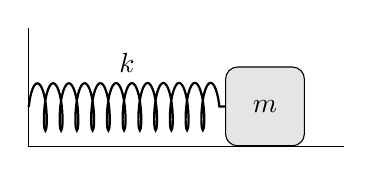
\begin{tikzpicture}
        %% Surface
        \draw (0,1.5) -- (0,0) -- (4,0);
        %% Mass
        \node[draw,fill=white!90!black,rectangle,rounded corners=1ex,minimum size=1cm,anchor=south] (M) at (3,0) {$m$};
        %% Spring and Rop
        \draw[thick,decoration={aspect=0.2,segment length=2.0mm,amplitude=3mm,coil},decorate] (0,0.5) -- (M.west) node[pos=0.5,yshift=3mm,anchor=south] {$k$};
    \end{tikzpicture}
    \end{center}
    If $k=\SI{50}{\newton\per\meter}$, $m=\SI{0.50}{\kilo\gram}$, $d=\SI{10}{\centi\meter}$,
        and the coefficient of kinetic friction between the block and the horizontal surface is equal to \num{0.25},
        determine the speed of the block when it first passes through the position for which the spring is unstretched.
    \begin{multicols}{3}
    \begin{choices}
        \wrongchoice{\SI{92}{\centi\meter\per\second}}
        \wrongchoice{\SI{61}{\centi\meter\per\second}}
      \correctchoice{\SI{71}{\centi\meter\per\second}}
        \wrongchoice{\SI{82}{\centi\meter\per\second}}
        \wrongchoice{\SI{53}{\centi\meter\per\second}}
    \end{choices}
    \end{multicols}
\end{question}
}

\element{serway-mc}{
\begin{question}{serway-ch08-q32}
    A \SI{2.0}{\kilo\gram} block sliding on a rough horizontal surface is attached to one end of a horizontal spring ($k=\SI{250}{\newton\per\meter}$) which has its other end fixed. 
    The block passes through the equilibrium position with a speed of \SI{2.6}{\meter\per\second} and first comes to rest at a displacement of \SI{0.20}{\meter} from equilibrium. 
    What is the coefficient of kinetic friction between the block and the horizontal surface?
    \begin{multicols}{3}
    \begin{choices}
        \wrongchoice{\num{0.32}}
      \correctchoice{\num{0.45}}
        \wrongchoice{\num{0.58}}
        \wrongchoice{\num{0.19}}
        \wrongchoice{\num{0.26}}
    \end{choices}
    \end{multicols}
\end{question}
}

\element{serway-mc}{
\begin{question}{serway-ch08-q33}
    In a given displacement of a particle,
        its kinetic energy increases by \SI{25}{\joule} while its potential energy decreases by \SI{10}{\joule}. 
    Determine the work of the nonconservative forces acting on the particle during this displacement.
    \begin{multicols}{3}
    \begin{choices}
        \wrongchoice{\SI{-15}{\joule}}
        \wrongchoice{\SI{+35}{\joule}}
      \correctchoice{\SI{+15}{\joule}}
        \wrongchoice{\SI{-35}{\joule}}
        \wrongchoice{\SI{+55}{\joule}}
    \end{choices}
    \end{multicols}
\end{question}
}

\element{serway-mc}{
\begin{question}{serway-ch08-q34}
    A particle is acted upon by only two forces,
        one conservative and one nonconservative,
        as it moves from point $A$ to point $B$. 
    The kinetic energies of the particle at points $A$ and $B$ are equal if:
    \begin{choices}
      \correctchoice{the sum of the works of the two forces is zero.}
        \wrongchoice{the work of the conservative force is equal to the work of the nonconservative force.}
        \wrongchoice{the work of the conservative force is zero.}
        \wrongchoice{the work of the nonconservative force is zero.}
        \wrongchoice{None of the above.}
    \end{choices}
\end{question}
}

\element{serway-mc}{
\begin{question}{serway-ch08-q35}
    A \SI{1.2}{\kilo\gram} mass is projected down a rough circular track (radius = \SI{2.0}{\meter}) as shown.
    \begin{center}
    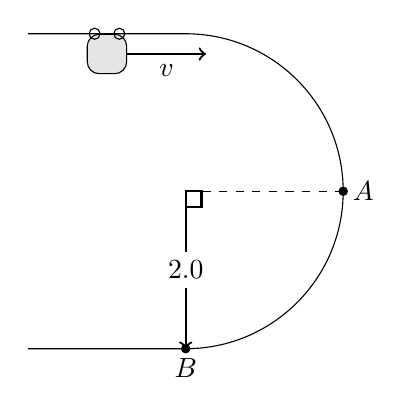
\begin{tikzpicture}
        %% Surface
        \draw (-2,2) -- (0,2) arc (90:-90:2) -- (-2,-2);
        %% Labels
        \draw[dashed] (0,0) -- ++(0:2);
        \draw[thick,->] (0,0) -- ++(270:2) node[anchor=center,fill=white,pos=0.5] {\SI{2.0}{\meter}};
        \draw[thick] (0,0) -- (0,-0.2) -- (0.2,-0.2) -- (0.2,0) -- cycle;
        \draw[fill] (0:2) circle (1.5pt) node[anchor=west] {$A$};
        \draw[fill] (270:2) circle (1.5pt) node[anchor=north] {$B$};
        %% Cart
        \node[draw,fill=white!90!black,rectangle,rounded corners=1ex,minimum size=0.5cm,anchor=north] (M) at (-1,2) {};
        \draw (M.north west) ++(0:0.1) circle (2pt);
        \draw (M.north east) ++(180:0.1) circle (2pt);
        \draw[thick,->] (M.east) -- ++(0:1) node[anchor=north,pos=0.5] {$v$};
    \end{tikzpicture}
    \end{center}
    The speed of the mass at point $A$ is \SI{3.2}{\meter\per\second},
        and at point $B$, it is \SI{6.0}{\meter\per\second}.
    How much work is done on the mass between $A$ and $B$ by the force of friction?
    \begin{multicols}{3}
    \begin{choices}
        \wrongchoice{\SI{-8.0}{\joule}}
        \wrongchoice{\SI{-7.3}{\joule}}
      \correctchoice{\SI{-8.1}{\joule}}
        \wrongchoice{\SI{-6.6}{\joule}}
        \wrongchoice{\SI{-24}{\joule}}
    \end{choices}
    \end{multicols}
\end{question}
}

\element{serway-mc}{
\begin{question}{serway-ch08-q36}
    A \SI{1.2}{\kilo\gram} mass is projected up a rough circular track (radius = \SI{0.80}{\meter}) as shown.
    \begin{center}
    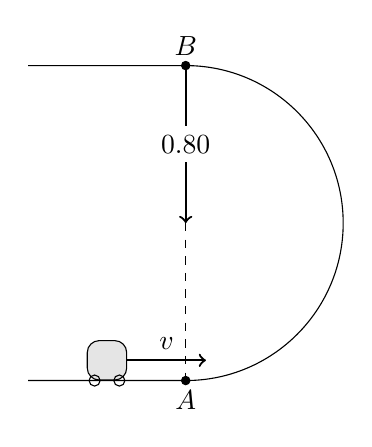
\begin{tikzpicture}
        %% Surface
        \draw (-2,2) -- (0,2) arc (90:-90:2) -- (-2,-2);
        %% Labels
        \draw[thick,->] (0,2) -- ++(270:2) node[anchor=center,fill=white,pos=0.5] {\SI{0.80}{\meter}};
        \draw[dashed] (0,0) -- ++(270:2);
        %\draw[thick] (0,0) -- (0,-0.2) -- (0.2,-0.2) -- (0.2,0) -- cycle;
        \draw[fill] (0,-2) circle (1.5pt) node[anchor=north] {$A$};
        \draw[fill] (0,2) circle (1.5pt) node[anchor=south] {$B$};
        %% Cart
        \node[draw,fill=white!90!black,rectangle,rounded corners=1ex,minimum size=0.5cm,anchor=south] (M) at (-1,-2) {};
        \draw (M.south west) ++(0:0.1) circle (2pt);
        \draw (M.south east) ++(180:0.1) circle (2pt);
        \draw[thick,->] (M.east) -- ++(0:1) node[anchor=south,pos=0.5] {$v$};
    \end{tikzpicture}
    \end{center}
    The speed of the mass at point $A$ is \SI{8.4}{\meter\per\second},
        and at point $B$, it is \SI{5.6}{\meter\per\second}. 
    How much work is done on the mass between $A$ and $B$ by the force of friction?
    \begin{multicols}{3}
    \begin{choices}
        \wrongchoice{\SI{-2.7}{\joule}}
        \wrongchoice{\SI{-8.8}{\joule}}
      \correctchoice{\SI{-4.7}{\joule}}
        \wrongchoice{\SI{-6.7}{\joule}}
        \wrongchoice{\SI{-19}{\joule}}
    \end{choices}
    \end{multicols}
\end{question}
}

\element{serway-mc}{
\begin{question}{serway-ch08-q37}
    A \SI{3.0}{\kilo\gram} mass is dropped from the edge of a \SI{50}{\meter} tall building with an initial speed of zero. 
    The mass strikes the ground with a downward velocity of \SI{25}{\meter\per\second}.
    How much work is done on the mass by air resistance between the point where it is dropped and the point where it strikes the ground?
    \begin{multicols}{3}
    \begin{choices}
        \wrongchoice{\SI{-0.46}{\kilo\joule}}
      \correctchoice{\SI{-0.53}{\kilo\joule}}
        \wrongchoice{\SI{-0.61}{\kilo\joule}}
        \wrongchoice{\SI{-0.38}{\kilo\joule}}
        \wrongchoice{\SI{-0.81}{\kilo\joule}}
    \end{choices}
    \end{multicols}
\end{question}
}

\element{serway-mc}{
\begin{question}{serway-ch08-q38}
    A \SI{2.0}{\kilo\gram} mass is projected vertically upward from ground level with an initial speed of \SI{30}{\meter\per\second}. 
    The mass rises to a maximum height of \SI{35}{\meter} above ground level. 
    How much work is done on the mass by air resistance between the point of projection and the point of maximum height?
    \begin{multicols}{3}
    \begin{choices}
      \correctchoice{\SI{-0.21}{\kilo\joule}}
        \wrongchoice{\SI{-0.47}{\kilo\joule}}
        \wrongchoice{\SI{-0.40}{\kilo\joule}}
        \wrongchoice{\SI{-0.34}{\kilo\joule}}
        \wrongchoice{\SI{-0.69}{\kilo\joule}}
    \end{choices}
    \end{multicols}
\end{question}
}

\element{serway-mc}{
\begin{question}{serway-ch08-q39}
    A \SI{25}{\kilo\gram} block on a horizontal surface is attached to a light spring (force constant = \SI{8.0}{\kilo\newton\per\meter}).
    The block is pulled \SI{10}{\centi\meter} to the right from its equilibrium position and released from rest. 
    When the block has moved \SI{2.0}{\centi\meter} toward its equilibrium position,
        its kinetic energy is \SI{12}{\joule}. 
    How much work is done by the frictional force on the block as it moves the \SI{2.0}{\centi\meter}?
    \begin{multicols}{3}
    \begin{choices}
        \wrongchoice{\SI{-4.0}{\joule}}
        \wrongchoice{\SI{-3.5}{\joule}}
      \correctchoice{\SI{-2.4}{\joule}}
        \wrongchoice{\SI{-2.9}{\joule}}
        \wrongchoice{\SI{-15}{\joule}}
    \end{choices}
    \end{multicols}
\end{question}
}

\element{serway-mc}{
\begin{question}{serway-ch08-q40}
    The two masses in the figure are released from rest. 
    After the \SI{3.0}{\kilo\gram} mass has fallen \SI{1.5}{\meter},
        it is moving with a speed of \SI{3.8}{\meter\per\second}. 
    \begin{center}
    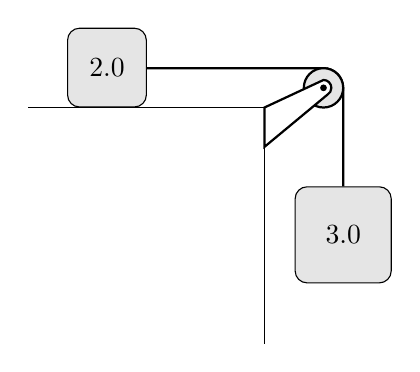
\begin{tikzpicture}
        %% Floor
        \draw (-3,0) -- (0,0) -- (0,-3);
        %% Mass
        \node[draw,fill=white!90!black,rectangle,rounded corners=1ex,minimum size=1.00cm,anchor=south] (A) at (-2,0) {\SI{2.0}{\kilo\gram}};
        \node[draw,fill=white!90!black,rectangle,rounded corners=1ex,minimum size=1.22cm,anchor=north] (B) at (1,-1) {\SI{3.0}{\kilo\gram}};
        %% Rope and Pully
        \draw[thick] (A.south east) ++(90:0.5) -- (0.75,0.5) arc(90:0:0.25) -- (B.north);
        \draw[thick,fill=white!90!black] (0.75,0.25) circle (0.25); 
        \draw[thick,fill=white] (0,0) -- (0.75,0.35) arc (90:-60:0.1) -- (0,-0.5) -- cycle;
        \draw[fill] (0.75,0.25) circle (1pt);
    \end{tikzpicture}
    \end{center}
    How much work is done during this time interval by the frictional force on the \SI{2.0}{\kilo\gram} mass?
    \begin{multicols}{3}
    \begin{choices}
        \wrongchoice{\SI{-12}{\joule}}
        \wrongchoice{\SI{-17}{\joule}}
        \wrongchoice{\SI{-20}{\joule}}
      \correctchoice{\SI{-8.0}{\joule}}
        \wrongchoice{\SI{-28}{\joule}}
    \end{choices}
    \end{multicols}
\end{question}
}

\element{serway-mc}{
\begin{question}{serway-ch08-q41}
    A \SI{2.0}{\kilo\gram} block is projected down a plane that makes an angle of \ang{20} with the horizontal with an initial kinetic energy of \SI{2.0}{\joule}. 
    If the coefficient of kinetic friction between the block and plane is \num{0.40},
        how far will the block slide down the plane before coming to rest?
    \begin{multicols}{3}
    \begin{choices}
      \correctchoice{\SI{3.0}{\meter}}
        \wrongchoice{\SI{1.8}{\meter}}
        \wrongchoice{\SI{0.30}{\meter}}
        \wrongchoice{\SI{1.0}{\meter}}
        \wrongchoice{\SI{1.3}{\meter}}
    \end{choices}
    \end{multicols}
\end{question}
}

\element{serway-mc}{
\begin{question}{serway-ch08-q42}
    A large spring is used to stop the cars after they come down the last hill of a roller coaster. 
    The cars start at rest at the top of the hill and are caught by a mechanism at the instant their velocities at the bottom are zero. 
    \begin{center}
    \hfill
    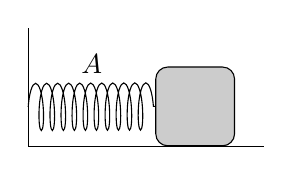
\begin{tikzpicture}
        \draw (0,1.5) -- (0,0) -- (3,0);
        \node[draw,fill=white!80!black,rectangle,rounded corners=1ex,minimum size=1cm,anchor=south] (M) at (2.12,0) {};
        \draw[decoration={aspect=0.2,segment length=1.4mm,amplitude=3mm,coil},decorate] (0,0.5) -- (M.west) node[pos=0.5,anchor=south,yshift=3mm] {$A$};
    \end{tikzpicture}
    \hfill
    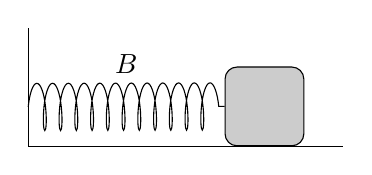
\begin{tikzpicture}
        \draw (0,1.5) -- (0,0) -- (4,0);
        \node[draw,fill=white!80!black,rectangle,rounded corners=1ex,minimum size=1cm,anchor=south] (M) at (3,0) {};
        \draw[decoration={aspect=0.2,segment length=2.0mm,amplitude=3mm,coil},decorate] (0,0.5) -- (M.west) node[pos=0.5,anchor=south,yshift=3mm] {$B$};
    \end{tikzpicture}
    \hfill~
    \end{center}
    Compare the compression of the spring, $x_A$,
        for a fully loaded car with that, $x_B$,
        for a lightly loaded car when $m_A = 2m_B$.
    \begin{multicols}{2}
    \begin{choices}
        \wrongchoice{$x_A = \dfrac{1}{2} x_B$}
        \wrongchoice{$x_A = x_B$}
      \correctchoice{$x_A = \sqrt{2} x_B$}
        \wrongchoice{$x_A = 2 x_B$}
        \wrongchoice{$x_A = 4 x_B$}
        %% added for symmetry
        \wrongchoice{$x_A = \dfrac{1}{\sqrt{2}} x_B$}
    \end{choices}
    \end{multicols}
\end{question}
}

\element{serway-mc}{
\begin{question}{serway-ch08-q43}
    A small lead sphere of mass $m$ is hung from a spring of spring constant $k$. 
    The gravitational potential energy of the system equals zero at the equilibrium position of the spring before the weight is attached. 
    The total mechanical energy of the system when the mass is hanging at rest is:
    \begin{multicols}{3}
    \begin{choices}
        \wrongchoice{$-kx^2$}
      \correctchoice{$-\dfrac{1}{2}kx^2$}
        \wrongchoice{zero}
        \wrongchoice{$+\dfrac{1}{2}kx^2$}
        \wrongchoice{$+kx^2$}
    \end{choices}
    \end{multicols}
\end{question}
}

\element{serway-mc}{
\begin{question}{serway-ch08-q44}
    Cubical blocks of mass $m$ and side $l$ are piled up in a vertical column. 
    The total gravitational potential energy of a column of three blocks is:
    \begin{multicols}{3}
    \begin{choices}
        \wrongchoice{$\dfrac{5}{2} mgl$}
        \wrongchoice{$3 mgl$}
      \correctchoice{$\dfrac{9}{2} mgl$}
        \wrongchoice{$6 mgl$}
        \wrongchoice{$9 mgl$}
        %% add one for symmetry
        \wrongchoice{$\dfrac{11}{2} mgl$}
    \end{choices}
    \end{multicols}
\end{question}
}

\element{serway-mc}{
\begin{question}{serway-ch08-q45}
    An all-terrain vehicle of \SI{2000}{\kilo\gram} mass moves up a \ang{15.0} slope at a constant velocity of \SI{6.00}{\meter\per\second}. 
    The rate of change of gravitational potential energy with time is:
    \begin{multicols}{3}
    \begin{choices}
        \wrongchoice{\SI{5.25}{\kilo\watt}}
        \wrongchoice{\SI{24.8}{\kilo\watt}}
      \correctchoice{\SI{30.4}{\kilo\watt}}
        \wrongchoice{\SI{118}{\kilo\watt}}
        \wrongchoice{\SI{439}{\kilo\watt}}
    \end{choices}
    \end{multicols}
\end{question}
}

\element{serway-mc}{
\begin{question}{serway-ch08-q46}
    A pendulum bob has potential energy $U_0$ when held taut in a horizontal position.
    The bob falls until it is \ang{30} away from the horizontal position,
        when it has potential energy $U_A$. 
    \begin{center}
    \begin{tikzpicture}
        %% Ceiling
        \node[anchor=south,fill,pattern=north east lines,minimum width=2cm, minimum height=0.05cm] at (0,0) {};
        \draw (-1,0) -- (1,0);
        %% Pivot
        \draw[fill] (-2pt,0) -- (-2pt,-2pt) arc (180:360:2pt) -- (2pt,0) --cycle;
        \draw (0,-2pt) -- ++(0:2) node[pos=1.0,anchor=west] {$U_O$};
        \draw (0,-2pt) -- ++(-30:2) node[anchor=north west] {$U_A$};
        \draw (0,-2pt) -- ++(270:2) node[anchor=north] {$U_B$};
    \end{tikzpicture}
    \end{center}
    It continues to fall until the string is vertical,
        when it has potential energy $U_B$. 
    Compare its potential energies at $O$, $A$, and $B$.
    \begin{choices}
        \wrongchoice{$U_O = U_A = U_B$}
        \wrongchoice{$U_A – U_B = 2 U_0$}
      \correctchoice{$U_A – U_B = U_0 - U_A$}
        \wrongchoice{$U_O = U_B = 2 U_A$}
        \wrongchoice{$U_O – U_A = 2 (U_A - U_B)$}
    \end{choices}
\end{question}
}

\element{serway-mc}{
\begin{question}{serway-ch08-q47}
    A spring with spring constant $k=\SI{800}{\newton\per\meter}$ is compressed \SI{12}{\centi\meter} from its equilibrium position. 
    A spring with spring constant $k=\SI{400}{\newton\per\meter}$ has the same elastic potential energy as the first spring when its extension is:
    \begin{multicols}{3}
    \begin{choices}
        %% changed cm to m
        \wrongchoice{\SI{0.060}{\meter}}
        \wrongchoice{\SI{0.085}{\meter}}
        \wrongchoice{\SI{0.12}{\meter}}
      \correctchoice{\SI{0.17}{\meter}}
        \wrongchoice{\SI{0.24}{\meter}}
    \end{choices}
    \end{multicols}
\end{question}
}

\element{serway-mc}{
\begin{question}{serway-ch08-q48}
    A spring with spring constant $k=\SI{800}{\newton\per\meter}$ is extended \SI{12}{\centi\meter} from its equilibrium position. 
    A spring with \SI{6.0}{\centi\meter} extension from equilibrium will have the same potential energy as the first spring if its spring constant is
    \begin{multicols}{2}
    \begin{choices}
        \wrongchoice{\SI{200}{\newton\per\meter}}
        \wrongchoice{\SI{400}{\newton\per\meter}}
        \wrongchoice{\SI{800}{\newton\per\meter}}
        \wrongchoice{\SI{1600}{\newton\per\meter}}
      \correctchoice{\SI{3200}{\newton\per\meter}}
    \end{choices}
    \end{multicols}
\end{question}
}

\element{serway-mc}{
\begin{question}{serway-ch08-q49}
    A champion athlete can produce one horsepower (\SI{746}{\watt}) for a short period of time. 
    If a \SI{70}{\kilo\gram} athlete were to bicycle to the summit of a \SI{500}{\meter} high mountain while expending power at this rate, she would have used at least \rule[-0.1pt]{4em}{0.1pt} of energy.
    \begin{multicols}{2}
    \begin{choices}
        \wrongchoice{\SI{746}{\joule}}
      \correctchoice{\SI{3.43e5}{\joule}}
        \wrongchoice{\SI{3.73e5}{\joule}}
        \wrongchoice{\SI{7.46e5}{\joule}}
        \wrongchoice{\SI{2.61e7}{\joule}}
    \end{choices}
    \end{multicols}
\end{question}
}

\element{serway-mc}{
\begin{question}{serway-ch08-q50}
    A champion athlete can produce one horsepower (\SI{746}{\watt}) for a short period of time. 
    If a \SI{70}{\kilo\gram} athlete were to bicycle to the summit of a \SI{500}{\meter} high mountain while expending power at this rate, she would reach the summit in:
    \begin{multicols}{3}
    \begin{choices}
        \wrongchoice{\SI{1}{\second}}
      \correctchoice{\SI{460}{\second}}
        \wrongchoice{\SI{500}{\second}}
        \wrongchoice{\SI{1000}{\second}}
        \wrongchoice{\SI{35 000}{\second}}
    \end{choices}
    \end{multicols}
\end{question}
}

\element{serway-mc}{
\begin{question}{serway-ch08-q51}
    A champion athlete can produce one horsepower (\SI{746}{\watt}) for a short period of time. 
    The number of \SI{16}{\centi\meter} high steps a \SI{70}{\kilo\gram} athlete could ascend in one minute while expending one horsepower is:
    \begin{multicols}{3}
    \begin{choices}
        \wrongchoice{\num{4}}
        \wrongchoice{\num{7}}
        \wrongchoice{\num{65}}
      \correctchoice{\num{408}}
        \wrongchoice{\num{4567}}
    \end{choices}
    \end{multicols}
\end{question}
}

\element{serway-mc}{
\begin{question}{serway-ch08-q52}
    Objects $A$ and $B$, of mass $M$ and $2M$ respectively,
        are each pushed a distance $d$ straight up an inclined plane by a force $F$ parallel to the plane. 
    The coefficient of kinetic friction between each mass and the plane has the same value $\mu_k$. 
    At the highest point,
    \begin{choices}
        \wrongchoice{$K_A = Fd = K_B$}
        \wrongchoice{$K_A = \left(F-\mu_k Mg\cos\theta\right)d$; \\
                     $K_B = \left(F-2\mu_k Mg\cos\theta\right)d$}
        \wrongchoice{$K_A = \left(F-Mg\sin\theta\right)d$; \\
                     $K_B = \left(F-2Mg\sin\theta\right)d$}
        \wrongchoice{$K_A = \left(F-Mg\sin\theta-\mu_k Mg\cos\theta\right)d$; \\
                     $K_B = \left(F-Mg\sin\theta-\mu_k Mg\cos\theta\right)d$}
      \correctchoice{$K_A = \left(F-Mg\sin\theta-\mu_k Mg\cos\theta\right)d$; \\
                     $K_B = \left(F-2Mg\sin\theta-2\mu_k Mg\cos\theta\right)d$}
    \end{choices}
\end{question}
}

\element{serway-mc}{
\begin{question}{serway-ch08-q53}
    As an object moves from point $A$ to point $B$ only two forces act on it:
        one force is nonconservative and does \SI{-30}{\joule} of work,
        the other force is conservative and does \SI{+50}{\joule} of work. 
    Between $A$ and $B$,
    \begin{choices}
      \correctchoice{the kinetic energy of object increases, mechanical energy increases.}
        \wrongchoice{the kinetic energy of object decreases, mechanical energy increases.}
        \wrongchoice{the kinetic energy of object decreases, mechanical energy decreases.}
        \wrongchoice{the kinetic energy of object increases, mechanical energy decreases.}
        \wrongchoice{None of the provided.}
    \end{choices}
\end{question}
}

\element{serway-mc}{
\begin{question}{serway-ch08-q54}
    As an object moves from point $A$ to point $B$ only two forces act on it:
        one force is conservative and does \SI{-70}{\joule} of work,
        the other force is nonconservative and does \SI{+50}{\joule} of work. 
    Between $A$ and $B$,
    \begin{choices}
        \wrongchoice{the kinetic energy of object increases, mechanical energy decreases.}
      \correctchoice{the kinetic energy of object decreases, mechanical energy decreases.}
        \wrongchoice{the kinetic energy of object decreases, mechanical energy increases.}
        \wrongchoice{the kinetic energy of object increases, mechanical energy increases.}
        \wrongchoice{None of the above.}
    \end{choices}
\end{question}
}

\element{serway-mc}{
\begin{question}{serway-ch08-q55}
    An astronaut tosses a ball out in space where gravitational forces may be neglected. 
    What will happen to the ball?
    \begin{choices}
        \wrongchoice{It will stop as soon as the force the astronaut gave it is used up.}
        \wrongchoice{It will stop when the energy the astronaut gave it runs out.}
        \wrongchoice{It will stop after a short time because there is no gravity to keep it moving.}
        \wrongchoice{It will move in a circle like a boomerang.}
      \correctchoice{It will be slowed down very gradually by collisions with molecules in space.}
    \end{choices}
\end{question}
}

\element{serway-mc}{
\begin{question}{serway-ch08-q56}
    Which of the following is a conservative force? 
    (All refer to a car on a slope.)
    \begin{choices}
        \wrongchoice{The force you exert on the car pushing it uphill.}
        \wrongchoice{The force exerted by rain drops falling on the car.}
        \wrongchoice{The frictional force of the road on the car.}
      \correctchoice{The gravitational force acting on the car.}
        \wrongchoice{The force you exert on the car (pushing it uphill) after it starts to slide downhill.}
    \end{choices}
\end{question}
}

\element{serway-mc}{
\begin{question}{serway-ch08-q57}
    For a force to be a conservative force,
        when applied to a single test body:
    \begin{choices}
        \wrongchoice{it must have the same value at all points in space.}
        \wrongchoice{it must have the same direction at all points in space.}
        \wrongchoice{it must be parallel to a displacement in any direction.}
        %% NOTE: the bottom two are too similar
        %\wrongchoice{equal work must be done in equal displacements.}
      \correctchoice{no work must be done for motion in closed paths.}
    \end{choices}
\end{question}
}

\element{serway-mc}{
\begin{question}{serway-ch08-q58}
    The force a spring exerts on a body is a conservative force because:
    \begin{choices}
        \wrongchoice{a spring always exerts a force opposite to the displacement of the body.}
        \wrongchoice{a spring always exerts a force parallel to the displacement of the body.}
        \wrongchoice{the work a spring does on a body is equal for compressions and extensions of equal magnitude.}
        \wrongchoice{the work a spring does on a body is equal and opposite for compressions and extensions of equal magnitude.}
      \correctchoice{the net work a spring does on a body is zero when the body returns to its initial position.}
    \end{choices}
\end{question}
}

\element{serway-mc}{
\begin{question}{serway-ch08-q59}
    Identical masses $m$ are attached to identical springs of spring constant $k$ suspended from the ceiling. 
    With both masses hanging in their equilibrium positions,
        mass $A$ is pulled down \SI{10}{\centi\meter} and released while mass $B$ is pushed up \SI{10}{\centi\meter} and released. 
    Which statement is correct?
    \begin{choices}
      \correctchoice{Mass $A$ will travel a smaller distance to its highest point than mass $B$ will travel to its lowest point.}
        \wrongchoice{Mass $A$ will travel a greater distance to its highest point than mass $B$ will travel to its lowest point.}
        \wrongchoice{Masses $A$ and $B$ will travel equal distances between their highest and lowest points.}
        \wrongchoice{More work was done on mass $A$ by the extending force than on mass $B$ by the compressing force.}
        \wrongchoice{The total work done on mass $A$ by the extending force was equal to the total work done on mass $B$ by the compressing force.}
    \end{choices}
\end{question}
}

\element{serway-mc}{
\begin{question}{serway-ch08-q60}
    Objects $A$ and $B$, of mass $M$ and $2M$ respectively,
        are each pushed a distance $d$ straight up an inclined plane by a force $F$ parallel to the plane. 
    The coefficient of kinetic friction between each mass and the plane has the same value $\mu_k$. 
    At the highest point,
    \begin{choices}
      \correctchoice{$K_A > K_B$}
        \wrongchoice{$K_A = K_B$}
        \wrongchoice{$K_A < K_B$}
        \wrongchoice{The work done by $F$ on $A$ is greater than the work done by $F$ on $B$.}
        \wrongchoice{The work done by $F$ on $A$ is less than the work done by $F$ on $B$.}
    \end{choices}
\end{question}
}

\element{serway-mc}{
\begin{question}{serway-ch08-q61}
    The equation below describes a physical situation:
    \begin{align*}
        &\dfrac{1}{2}\left(\SI{1.70}{\kilo\gram}\right)\left(\SI{3.30}{\meter\per\second}\right)^2 \\
        &\quad\quad + \left(\SI{1.70}{\kilo\gram}\right)\left(\SI{9.80}{\meter\per\second\squared}\right)\left(\SI{2.35}{\meter}\right)\sin\ang{30} \\
        &\quad = \left(\SI{1.70}{\kilo\gram}\right)\left(\SI{1.08}{\meter\per\second}\right)^2 \\
        &\quad\quad + \num{0.320}\left(\SI{1.70}{\kilo\gram}\right)\left(\SI{9.80}{\meter\per\second\squared}\right)\left(\SI{2.35}{\meter}\right)\cos\ang{30} \\
    \end{align*}
    Which description best fits the equation?
    \begin{choices}
        \wrongchoice{A \SI{1.70}{\kilo\gram} block slows down while sliding down a frictionless plane inclined at a \ang{30} angle.}
      \correctchoice{A \SI{1.70}{\kilo\gram} block slows down while sliding down a plane with $\mu_k=\num{0.320}$, with the plane inclined at a \ang{30} angle.}
        \wrongchoice{A \SI{1.70}{\kilo\gram} block slows down while sliding up a frictionless plane inclined at a \ang{30} angle.}
        %% Changed down to up
        \wrongchoice{A \SI{1.70}{\kilo\gram} block slows down while sliding up a plane with $\mu_k=\num{0.320}$, with the plane inclined at a \ang{30} angle.}
        \wrongchoice{A \SI{1.70}{\kilo\gram} block slides over the top of an inclined plane and then descends on the other side. Both planes, inclined at a \ang{30} angle, have $\mu_k=\num{0.320}$.}
    \end{choices}
\end{question}
}

\element{serway-mc}{
\begin{question}{serway-ch08-q62}
    %% NOTE: changed 0.800 kg to 0.500 kg
    A spring with spring constant \SI{800}{\newton\per\meter} compressed \SI{0.200}{\meter} is released and projects a \SI{0.500}{\kilo\gram} mass along a frictionless surface. 
    The mass reaches a surface area where $\mu_k=\num{0.400}$ and comes to a stop. 
    The following student solution contains at least one error. 
    What is the error?
    \begin{align*}
        &\dfrac{1}{2}\left(\SI{800}{\newton\per\meter}\right)\left(\SI{0.200}{\meter}\right)^2 = \\
        &\quad \left(\SI{0.500}{\kilo\gram}\right)\left(\SI{8.00}{\meter\per\second}\right)^2 \\
        &\quad\quad +\num{0.400}\left(\SI{0.500}{\kilo\gram}\right)\left(\SI{9.80}{\meter\per\second\squared}\right)\left(\SI{8.16}{\meter}\right)
    \end{align*}
    \begin{choices}
        \wrongchoice{The elastic potential energy is equal only to the kinetic energy on the right, and is never equal to the internal thermal energy.}
        \wrongchoice{The elastic potential energy is equal only to the internal thermal energy on the right, and is never equal to the kinetic energy.}
      \correctchoice{The elastic potential energy is equal to either the kinetic energy or the internal thermal energy on the right, but not to their sum.}
        \wrongchoice{Elastic potential energy cannot end up as work done by friction.}
        \wrongchoice{Work done by friction cannot end up as elastic potential energy.}
    \end{choices}
\end{question}
}

\element{serway-mc}{
\begin{question}{serway-ch08-q63}
    The solution to a problem is the equation below. Which description best fits this solution?
    \begin{align*}
        & \dfrac{1}{2}\left(\SI{500}{\newton\per\meter}\right)\left(\SI{0.120}{\meter}\right)^2 \\
        &\quad\quad-\left(\SI{2.00}{\kilo\gram}\right)\left(\SI{9.80}{\meter\per\second\squared}\right)^2\left(\SI{0.120}{\meter}\right) \\
        &\quad = \dfrac{1}{2}\left(\SI{2.00}{\kilo\gram}\right)\left(\SI{0.820}{\meter\per\second}\right)^2 \\
        &\quad\quad+\left(\SI{2.00}{\kilo\gram}\right)\left(\SI{9.80}{\meter\per\second\squared}\right)\left(\SI{0.0290}{\meter}\right)
    \end{align*}
    \begin{choices}
      \correctchoice{A vertical spring compressed \SI{0.120}{\meter} shoots a \SI{2.00}{\kilo\gram} mass \SI{2.90}{\meter} above the equilibrium position of the spring.}
        \wrongchoice{A vertical spring stretched \SI{0.120}{\meter} shoots a \SI{2.00}{\kilo\gram} mass \SI{9.10}{\meter} above the equilibrium position of the spring.}
        \wrongchoice{A vertical spring compressed \SI{0.120}{\meter} shoots a \SI{2.00}{\kilo\gram} mass \SI{12.0}{\centi\meter} above the equilibrium position of the spring.}
        \wrongchoice{A vertical spring compressed \SI{0.120}{\meter} shoots a \SI{2.00}{\kilo\gram} mass \SI{14.9}{\centi\meter} above the equilibrium position of the spring.}
        \wrongchoice{A \SI{2.00}{\kilo\gram} mass has fallen \SI{0.820}{\meter} and compressed the upper end of a vertical spring \SI{12.0}{\centi\meter} below the equilibrium position.}
    \end{choices}
\end{question}
}

\element{serway-mc}{
\begin{question}{serway-ch08-q64}
    As a result of friction between internal parts of an isolated system:
    \begin{choices}
        \wrongchoice{the total mechanical energy of the system increases.}
      \correctchoice{the total mechanical energy of the system decreases.}
        \wrongchoice{the total mechanical energy of the system remains the same.}
        \wrongchoice{the potential energy of the system increases but the kinetic energy remains the same.}
        \wrongchoice{the kinetic energy of the system increases but the potential energy of the system remains the same.}
    \end{choices}
\end{question}
}

\element{serway-mc}{
\begin{question}{serway-ch08-q65}
    A \SI{3.50}{\kilo\gram} block is pulled along a moving conveyor belt at a constant speed of \SI{0.500}{\meter\per\second} relative to a stationary observer while the belt moves at a constant speed of \SI{0.200}{\meter\per\second} in the same direction. 
    If the coefficient of kinetic friction is \num{0.400},
        the magnitude of the work done on the block by the force of friction in \SI{8.00}{\second} is:
    \begin{multicols}{3}
    \begin{choices}
        \wrongchoice{\SI{5.6}{\joule}}
        \wrongchoice{\SI{22.0}{\joule}}
      \correctchoice{\SI{32.9}{\joule}}
        \wrongchoice{\SI{54.8}{\joule}}
        \wrongchoice{\SI{76.8}{\joule}}
    \end{choices}
    \end{multicols}
\end{question}
}

\element{serway-mc}{
\begin{question}{serway-ch08-q66}
    A \SI{3.50}{\kilo\gram} block is pulled along a moving conveyor belt at a constant speed of \SI{0.500}{\meter\per\second} relative to a stationary observer while the belt moves at a constant speed of \SI{0.200}{\meter\per\second} in the opposite direction. 
    If the coefficient of kinetic friction is \num{0.400},
        the magnitude of the work done on the block by the force of friction in \SI{8.00}{\second} is:
    \begin{multicols}{3}
    \begin{choices}
        \wrongchoice{\SI{5.6}{\joule}}
        \wrongchoice{\SI{22.0}{\joule}}
        \wrongchoice{\SI{32.9}{\joule}}
        \wrongchoice{\SI{54.8}{\joule}}
      \correctchoice{\SI{76.8}{\joule}}
    \end{choices}
    \end{multicols}
\end{question}
}

\element{serway-mc}{
\begin{question}{serway-ch08-q67}
    Jane and Jake are looking at what happens to body 1 of mass $m$ and body 2 of mass $2m$,
        initially at rest, when equal forces are applied separately to the two bodies. 
    Jake says that equal forces applied for equal times do equal amounts of work on the two bodies. 
    Jane says that the two forces do equal amounts of work only if the two bodies move equal distances in the direction of the forces. 
    Which one, if either, is correct?
    \begin{choices}
        \wrongchoice{Jake, because the speed of body 1 is half the speed of body 2, but $m_1 v_1 = m_2 v_2$.}
      \correctchoice{Jane, because $v_2=\dfrac{v_1}{\sqrt{2}}$ so $mv^2$ is the same for both bodies.}
        \wrongchoice{Jake, because all bodies travel equal distances when equal forces are applied for equal times.}
        \wrongchoice{Jane, because it takes the same time for all bodies to travel equal distances when equal forces are involved.}
        \wrongchoice{Neither, because we can't compare the amounts of work done on bodies of different mass.}
    \end{choices}
\end{question}
}

\element{serway-mc}{
\begin{question}{serway-ch08-q68}
    The same force $F$ is applied horizontally to bodies 1, 2, 3 and 4, of masses $m$, $2m$, $3m$ and $4m$, initially at rest and on a frictionless surface, until each body has traveled distance $d$. 
    The correct listing of the magnitudes of the velocities of the bodies, $v_1$, $v_2$, $v_3$, and $v_4$ is:
    \begin{choices}
        \wrongchoice{$v_4 = \sqrt{\dfrac{4}{3}} v_3 = \sqrt{\dfrac{3}{2}} v_2 = 2v_1$}
        \wrongchoice{$v_4 = v_2 >  v_3 = v_1$}
      \correctchoice{$v_1 = \sqrt{2} v_2 = \sqrt{3} v_3 = 2 v_4$}
        \wrongchoice{$v_1 = 2 v_2 = 3 v_3 = 4 v_4$}
        \wrongchoice{$v_4 = \dfrac{3}{4} v_3 = \dfrac{2}{3} v_2 = \dfrac{1}{2} v_1$}
    \end{choices}
\end{question}
}

\element{serway-mc}{
\begin{question}{serway-ch08-q69}
    Any change of the energy of a system occurs because of:
    \begin{choices}[o]
      \correctchoice{energy transfer across the boundaries of the system.}
        \wrongchoice{combustion of fuels within the system.}
        \wrongchoice{radioactive decay of elements within the system.}
        \wrongchoice{all of the above.}
        \wrongchoice{only (b) and (c) above.}
    \end{choices}
\end{question}
}

\element{serway-mc}{
\begin{question}{serway-ch08-q70}
    Two masses, $M_A$ and $M_B$,
        with $M_B=2M_A$, are released at the same time and allowed to fall straight down. 
    Neglect air resistance. 
    When we compare their kinetic energies after they have fallen equal distances, we find that:
    \begin{multicols}{2}
    \begin{choices}
        \wrongchoice{$K_B = K_A$}
      \correctchoice{$K_B = 2 K_A$}
        \wrongchoice{$K_B = 4 K_A$}
        \wrongchoice{$K_A = 2 K_B$}
        \wrongchoice{$K_A = 4 K_B$}
    \end{choices}
    \end{multicols}
\end{question}
}

\element{serway-mc}{
\begin{question}{serway-ch08-q71}
    Two masses, $M_A$ and $M_B$, with $M_B = 2M_A$,
        are released at the same time and allowed to fall straight down. 
    Neglect air resistance. 
    When we compare their kinetic energies after they have fallen for equal times, we find that:
    \begin{multicols}{2}
    \begin{choices}
        \wrongchoice{$K_B = K_A$}
      \correctchoice{$K_B = 2 K_A$}
        \wrongchoice{$K_B = 4 K_A$}
        \wrongchoice{$K_A = 2 K_B$}
        \wrongchoice{$K_A = 4 K_B$}
    \end{choices}
    \end{multicols}
\end{question}
}

\endinput


